\documentclass[tikz, border = 1 cm]{standalone}

%%%%%%%%%%%%%%
\usepackage{bm}
\usepackage{tikz}
\usetikzlibrary{calc}
%%%%%%%%%%%%%%

%%%%%%%%%%%%%%
\definecolor{blue1}	{RGB}{0,177,234}
\definecolor{purple1}	{RGB}{89,89,171}
\definecolor{gray2}	{RGB}{129,135,141}
%%%%%%%%%%%%%%

%%%%%%%%%%%%%%
%%%%%%%%%%%%%%
%%%%%%%%%%%%%%
\begin{document}

%%%%%%%%%%%%%%
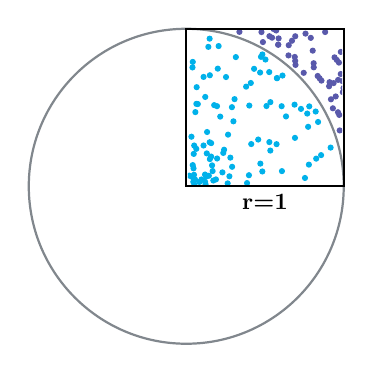
\begin{tikzpicture}
	\draw[thick,draw=gray2] (0,0) circle (2cm);
	\draw[thick] (0,0) rectangle (2,2);
	\newcommand{\points}{
		\foreach \x in {1,...,100}{
			\pgfmathrandominteger{\r}{3}{55}
			\pgfmathrandominteger{\t}{3}{87}
			\pgfpathcircle{\pgfpointpolar{\t}{\r}}{0.9pt}
			\color{blue1}
			\pgfsetstrokecolor{blue1}
			\pgfusepath{stroke, fill}
		}	
		\foreach \x in {1,...,100}{
			\pgfmathrandominteger{\r}{59}{76}
			\pgfmathrandominteger{\t}{2}{88}
			\pgfpathcircle{\pgfpointpolar{\t}{\r}}{0.9pt}
			\color{purple1}
			\pgfsetstrokecolor{purple1}
			\pgfusepath{stroke, fill}
		}
	}
	\newcommand{\carre}{(0.02,0.02) rectangle (1.98,1.98)}
	\begin{scope}
		\clip \carre;
		\points;
	\end{scope}
	\node[thick,scale=0.85] at (1,-0.2) {\textbf{r=1}};
\end{tikzpicture}
%%%%%%%%%%%%%%

\end{document}